\documentclass[a4paper]{article}
\usepackage[pdftex]{graphicx}
\usepackage[utf8]{inputenc}
\usepackage{enumerate}
\usepackage{siunitx}
\sisetup{locale=DE} 
\usepackage{icomma}
\usepackage{amssymb}
\usepackage{tikz}
\usepackage{href-ul}
\hypersetup{
	colorlinks=true,
	linkcolor=blue,
	urlcolor=blue}
\usepackage{geometry}
\geometry{a4paper, top=15mm, left=15mm, right=15mm, bottom=15mm,
	headsep=10mm, footskip=12mm}

\begin{document}
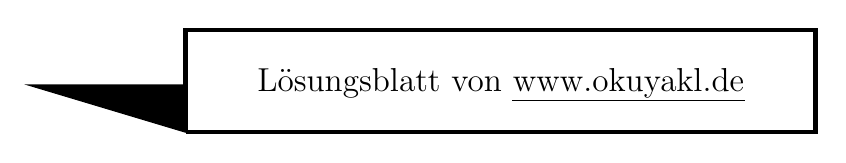
\begin{tikzpicture}(10,3)
	\draw[ultra thick](2,0) --(10,0) -- (10,1.3) --(2,1.3) -- (2,0);
	\draw[fill=black](2,0)-- (0,.6) -- (2,.6) -- (2,0);
	\node at (6,.6) {\large Lösungsblatt von \href{https://www.okuyakl.de}{www.okuyakl.de}};
\end{tikzpicture}
\vspace{0.5 cm}


\noindent {\bf Aufgabe 1. a)}\\
\begin{minipage}{0.4\textwidth}
Zunächst wandeln wir die Frequenzen in Schwingungsdauern mit der Formel $T={1\over f}$ um,
dann tragen wir die Schwingungsdauer $T$ über  der Fadenlänge $l$ auf:
\end{minipage}
\hfill
\begin{minipage}{0.6\textwidth}
\includegraphics[width=5 cm]{pendia119}
\end{minipage}
\vspace{0.5 cm}

\noindent {\bf Aufgabe 1. b)}\\
Aus dem Diagramm lesen wir ab: $$T=\SI{1,5}{\second} \quad \Rightarrow \quad l=\SI{0,57}{\meter}$$
\vspace{0.5 cm}

\noindent {\bf Aufgabe 1. c)}\\
Die Schwingungsdauer hängt für kleine Auslenkungen nur von der Länge des Fadens ab, nicht von der Masse des angehängten Gewichts.
\vspace{0.5 cm}

\noindent {\bf Aufgabe 1. d)}\\
Wir rechnen: (N=Anzahl der Schwingungen) 
$$N=\SI{24}{\second} \cdot \SI{0,5}{\hertz} = 12 $$
\vspace{0.5 cm}

\noindent {\bf Aufgabe 2. a)}\\
Bei einer harmonischen Schwingung...

\begin{itemize}
	\item ...ist die Schwingungsdauer immer gleich, unabhängig von der Amplitude.
	\item ...ist die rücktreibende Kraft proportional zur Auslenkung.
\end{itemize}
\vspace{0.5 cm}

\noindent{\bf Aufgabe 2. b)}\\
1. Möglichkeit; Berechnung aus der Masse und der Federhärte: 
$$ T = 2 \pi \cdot \sqrt{m \over D} = 2 \pi \cdot \sqrt{\SI{0,44}{\kilogram} \over  \SI{12}{\newton\over\meter}} = \SI{1,2}{\second}$$
2. Möglichkeit; Berechnung aus der Anzahl der Schwingungen pro Zeiteinheit:
$$ T= {\SI{12}{\second} \over 10} = \SI{1,2}{\second}$$
Die Ergebnisse sind gleich; die Frequenz beträgt in beiden Fällen
$$f= {1 \over T}= \SI{0,83}{\hertz}$$

\newpage
\noindent{\bf Aufgabe 2. c)}\\
\begin{minipage}{0.5\textwidth}
Die Schwingung beginnt während der Abwärtsbewegung durch die Ruhelage. Daraus folgt: $v(t)$ ist eine Kosinusfunktion mit negativem Vorzeichen:
$$v(t)= - \SI{0,30}{\meter\over\second} \cdot \cos{\left( {2\pi \over \SI{1,2}{\second}}\cdot t \right)}$$
$$v(\SI{7,9}{\second})=\SI{-0,23}{\meter\over\second}$$
Die maximale Beschleunigung tritt in den Umkehrpunkten auf, wenn die Geschwindigkeit Null ist.
\end{minipage}
\hfill
\begin{minipage}{0.5\textwidth}
\includegraphics[width=6 cm]{scwv94.pdf}
\end{minipage}
\vspace{0.5 cm}

\noindent{\bf Aufgabe 2. d)}\\
Es gilt der Energieerhaltungssatz. Die Spannungsenergie in den Umkehrpunkten ist gleich der kinetischen Energie bei $v_{max}$:
$$
\renewcommand{\arraystretch}{2}
\begin{array}{rcll}
 {1 \over 2} D \cdot \hat{x}^2 &=&   {1 \over 2} m \cdot v_{max}^2 & |\cdot 2 \qquad : D \\
  \hat{x}^2 &=& {m \over D} \cdot v_{max}^2 & | \sqrt{\qquad}\\
  \hat{x} &=& \sqrt{m \over D} \cdot  v_{max} \\
  \hat{x} &=& \sqrt{\SI{0,44}{\kilogram} \over \SI{12}{\newton\over\meter}} \cdot  \SI{0,3}{\meter\over\second} &=\SI{0,057}{\meter} \approx \SI{6}{\centi\meter}
\end{array}
$$
\vspace{0.5 cm}

\noindent{\bf Aufgabe 2. e)}\\
Für die Federkraft gilt das Hooke'sche Gesetz, für die Beschleunigung der Trägheitssatz: 
$$F = - D \cdot \hat{x} = m \cdot a $$
$$ \Leftrightarrow a= -{D \over m} \cdot \hat{x} = {\SI{12}{\kilogram\over {\second^2}} \over \SI{0,44}{\kilogram}}\cdot \SI{0,057}{\meter} =  \SI{-1,6}{\meter \over{ \second^2}}$$
Der Betrag der Beschleunigung ist $\SI{1,6}{\meter \over{ \second^2}}$; sie ist nach unten gerichtet, weil das Vorzeichen negativ ist.
\vspace{0.5 cm}

\noindent{\bf Aufgabe 2. f)}\\
Wir stellen folgende Beziehung nach der Federhärte um:
$$
\renewcommand{\arraystretch}{2}
\begin{array}{rcll}
(*) \qquad T &=& 2 \pi \cdot \sqrt{m\over D} & |: 2 \pi \\
{T \over 2 \pi} &=& \sqrt{m\over D} & |()^2 \\
{T^2 \over 4 \pi^2} &=&  {m\over D} & |()^{-1} \\
{4 \pi^2 \over T^2} &=& {D\over m}  & |\cdot m \\
{4 \pi^2 \over T^2}\cdot m &=& D & =  \SI{7,7}{\newton\over\meter} 
\end{array}
$$
\vspace{0.5 cm}
\begin{minipage}{0.5\textwidth}
\noindent{\bf Aufgabe 3. a)}\\
Es gilt nach $(*)$:\\ 
$ T \sim \sqrt{m} \Rightarrow$ Verdoppelung der Schwingungsdauer wird durch Vervierfachung der Masse erreicht.
\vspace{0.5 cm}

\noindent{\bf Aufgabe 3. b)}\\
$F \sim D \Rightarrow$ Halbe Kraft bedeutet halbe Federhärte.
\end{minipage}
\begin{minipage}{0.5\textwidth}
\begin{center}
	\includegraphics[width=7 cm]{../../viecher/endcomic.pdf}
	
	Hier geht es zurück zum \href{https://www.okuyakl.de/phys/p10penL407/aa407.pdf}{Aufgabenblatt}
\end{center}
\end{minipage}
\end{document}

